\documentclass[conference]{IEEEtran}
\IEEEoverridecommandlockouts
\raggedbottom
\setlength{\textfloatsep}{6pt plus 2pt minus 2pt}
\setlength{\floatsep}{6pt plus 2pt minus 2pt}
\setlength{\intextsep}{6pt plus 2pt minus 2pt}
\setlength{\abovecaptionskip}{4pt}
\setlength{\belowcaptionskip}{2pt}

\usepackage{cite}
\usepackage{amsmath,amssymb}
\usepackage{mathptmx}
\usepackage{graphicx}
\usepackage{booktabs}
\usepackage{url}
\usepackage[table]{xcolor}
\usepackage{tikz}
\usetikzlibrary{shapes.geometric,arrows.meta,positioning,fit,backgrounds,calc,shadows}
\usepackage{pgfplots}
\pgfplotsset{compat=1.17}
\usepackage{algorithm}
\usepackage{algorithmic}
\renewcommand{\algorithmicrequire}{\textit{Require:}}
\renewcommand{\algorithmicensure}{\textit{Ensure:}}
\renewcommand{\algorithmicif}{\textit{if}}
\renewcommand{\algorithmicthen}{\textit{then}}
\renewcommand{\algorithmicelse}{\textit{else}}
\renewcommand{\algorithmicendif}{\textit{end if}}
\renewcommand{\algorithmicfor}{\textit{for}}
\renewcommand{\algorithmicforall}{\textit{for all}}
\renewcommand{\algorithmicdo}{\textit{do}}
\renewcommand{\algorithmicendfor}{\textit{end for}}
\renewcommand{\algorithmicwhile}{\textit{while}}
\renewcommand{\algorithmicendwhile}{\textit{end while}}
\renewcommand{\algorithmicrepeat}{\textit{repeat}}
\renewcommand{\algorithmicuntil}{\textit{until}}
\renewcommand{\algorithmicreturn}{\textit{return}}
\renewcommand{\algorithmicprint}{\textit{print}}
\usepackage[hidelinks]{hyperref}

\newcommand{\ph}[1]{{\color{red}\textbf{[#1]}}}

\begin{document}

\title{Realtime Web Attack Detection and Inline Blocking Using a Hybrid
Rule Based Transformer For Web Application Firewall}

\author{\IEEEauthorblockN{Priscilla Jospin G\IEEEauthorrefmark{1}\thanks{\IEEEauthorrefmark{1}Corresponding author.}}
\IEEEauthorblockA{Division of Data Science and Cyber Security\\
Karunya Institute of Technology and Sciences\\
Coimbatore, India\\
priscillajosin@karunya.edu.in}
\and
\IEEEauthorblockN{Rahul R}
\IEEEauthorblockA{Division of Data Science and Cyber Security\\
Karunya Institute of Technology and Sciences\\
Coimbatore, India\\
rahul@karunya.edu}
}

\maketitle

\begin{abstract}
Signature-based web application firewalls (WAFs) are easy to bypass with
obfuscated payloads. Transformer detectors report strong accuracy, yet
they are usually tested offline, without measuring latency or false
positives. We place a fine-tuned BERT model inside an Nginx sub-request
enforcement path, combine it with rules through a four-tier fusion policy,
and evaluate the full system on CSIC~2010. The model alone reaches
F1~$0.949$ at a $6.4\%$ false-positive rate (ROC--AUC~$0.974$), well above a
signature engine (F1~$0.567$) and close to a TF--IDF SVM, with a median GPU
inference time of $12.7$~ms. Six families of semantics-preserving mutation
evade the model on $0.12\%$ of blocked payloads and never evade the hybrid.
Because this gap is so small, mutation resistance cannot account for the
hybrid's higher false-positive rate ($22.9\%$ against $6.4\%$). We then ran
the CSIC-trained detector zero-shot on two other corpora. On SR-BH~2020 the
model alone flagged nearly all traffic (FPR~$1.00$) while the hybrid reached
F1~$0.971$. On real 2025 production traffic the result flipped: the model
recalled $99.9\%$ of attacks and the hybrid only $15.1\%$. The rule layer
can therefore help generalisation on one corpus and harm it on another, and
we report both outcomes.
\end{abstract}

\begin{IEEEkeywords}
web application firewall, transformer, BERT, inline enforcement, decision fusion.
\end{IEEEkeywords}

\section{Introduction}
SQL injection, cross-site scripting, path traversal and command injection
have stayed near the top of the OWASP Top Ten for years. The usual defence
is a web application firewall (WAF), a proxy that inspects each request and
drops the ones it judges malicious before the backend sees them. In most
deployments that judgement comes from signatures and regular expressions;
ModSecurity with the OWASP Core Rule Set~\cite{owaspcrs} is the standard
example. Rule sets are fast and easy to audit, yet they match strings
rather than meaning. An attacker can add an inline SQL comment, change
letter case or URL-encode a payload twice, and the request still does the
same thing on the server while the rule no longer fires. Tightening the
rules to cover such variants tends to block real users.

Transformer models~\cite{vaswani2017attention,devlin2019bert} offer a
different route, since a fine-tuned encoder can learn the structure of an
attack from examples instead of relying on hand-written patterns.
Published transformer classifiers report over $99\%$ accuracy on
CSIC~2010~\cite{wadbert2026,scireports2024novelxsssqli}. Most of these
studies, however, train and test on a fixed corpus and never run the model
as a firewall. Three questions stay open. How much latency does the model
add when every request has to wait for it? How many legitimate requests
does it block at a usable threshold? And does adding it to an existing rule
engine improve detection or make it worse?

To study these questions we built a WAF in which the transformer sits in
the live request path through Nginx's sub-request authorization, with no
change to the protected application. A four-tier fusion policy combines
fixed signatures and anomaly rules with banded model scores, plus an
endpoint safelist and a fail-open safeguard. We evaluate detection quality, an ablation, threshold sensitivity, inline
latency and adversarial evasion, and we test zero-shot transfer to two
further corpora. The two transfer results disagree. On SR-BH~2020 the model
on its own breaks down and the rule layer recovers it, while on newer
production traffic the rule layer cuts the hybrid's recall sharply.

\section{Related Work}
Kheddar et al.~\cite{kheddar2025survey} survey transformer and LLM methods
for intrusion detection. In practice most WAFs still rely on rule sets such
as OWASP CRS~\cite{owaspcrs}, and many machine-learning detectors use
handcrafted features that transfer poorly to new traffic, including a recent
decision-tree WAF tested in real time~\cite{mlwaf2025peerj}; our TF--IDF
baselines represent this group. Deep and transformer detectors now report
over $99\%$ within-corpus accuracy on SQLi and
XSS~\cite{scireports2024novelxsssqli,wadbert2026,zhou2025ewebguard}, and
domain-adapted or distilled
encoders~\cite{aghaei2022securebert,aghaei2025securebert2,sanh2019distilbert}
aim to lower inference cost. On the attack side,
WAF-A-MoLE~\cite{demetrio2020wafamole} showed that ML-based WAFs can be
bypassed with mutated payloads, and later work generated adversarial SQL
injections against commercial WAF services~\cite{advsqli2024} and
LLM-written XSS payloads and rules~\cite{genxss2025}. Few transformer-WAF
papers test against such mutations, and we found none that runs a
transformer behind a reverse proxy and reports the latency and
false-positive cost of doing so. Table~\ref{tab:compare} summarises these
differences.

\begin{table*}[t]
\centering
\caption{Comparison with representative prior work. Headline results are
each paper's own, on its own data and splits, and are therefore not
directly comparable to one another. \checkmark\ = evaluated in the cited
work; \textbf{---} = not reported there; ``part.'' = partially.}
\label{tab:compare}
\footnotesize
\setlength{\tabcolsep}{4pt}
\begin{tabular}{@{}llp{5.6cm}cccc@{}}
\toprule
Work & Approach & Headline result as reported & Inline & Latency & FPR ctrl. & Cross-data \\
\midrule
OWASP CRS~\cite{owaspcrs}              & Signature rules & Reference rule set (rules-only F1 $0.567$ here) & \checkmark & part. & manual & --- \\
Deep SQLi/XSS~\cite{scireports2024novelxsssqli} & Deep learning & Accuracy $99.77\%$ on CSIC~2010 & --- & --- & --- & --- \\
WADBERT~\cite{wadbert2026}             & Dual-channel BERT & F1 $99.63\%$ (CSIC), $99.50\%$ (SR-BH), trained per corpus & --- & --- & --- & --- \\
BERT--LSTM~\cite{liu2024bertlstm}      & BERT + LSTM     & Accuracy $0.973$, F1 $0.958$ on SQLi detection & --- & --- & --- & --- \\
ADL-WAF~\cite{adlwaf2025}              & Decision tree + SVM & Accuracy $99.88\%$, precision $100\%$, five datasets & --- & --- & part. & --- \\
WAF-A-MoLE~\cite{demetrio2020wafamole} & Evasion attack  & Mutates payloads past ML-based WAFs & --- & --- & --- & --- \\
\textbf{This work}                     & Rules + BERT, inline & F1 $0.949$, FPR $0.064$, $12.7$~ms median, $0.12\%$ evasion (hybrid $0\%$), two unseen corpora & \checkmark & \checkmark & \checkmark & \checkmark \\
\bottomrule
\end{tabular}
\end{table*}

Two points stand out in Table~\ref{tab:compare}. The cited detectors report
higher in-corpus scores than ours (F1 $99.63\%$ against $0.949$), but each is
an offline classifier tested on its own corpus, and none gives per-request
cost or false positives at a fixed threshold. Our system is the only one
evaluated on all four deployment properties. It blocks inline at a median
of $12.7$~ms ($82$ requests/s per process). Against the signature engine
alone it raises F1 from $0.567$ to $0.949$ and lowers FPR from $0.209$ to
$0.064$, and FPR drops to $0.026$ at a recall of $0.880$ with a higher
threshold. Mutation evasion is $0.12\%$ for the model and zero for the
hybrid, and the fused policy is tested on two unseen corpora. Part of our
lower in-corpus score is the cost of deduplicating CSIC~2010 before
splitting.

Within-corpus
studies~\cite{scireports2024novelxsssqli,wadbert2026} report accuracy or F1
above $99\%$ on CSIC~2010. CSIC~2010's benign traffic is templated, so a split that
does not deduplicate near-identical requests before partitioning can inflate
accuracy through leakage rather than generalisation; deduplication is
applied here before splitting specifically to avoid that, which may
account for part of the gap between the F1 reported here and those figures. Cross-dataset studies in network intrusion detection report a similar drop
when a model meets traffic from another
network~\cite{cantone2024crossdataset,venkatesan2026crossdataset}. They do
not test whether a rule layer can make up the loss, which is the question
Section~\ref{sec:crossdataset} examines for WAFs.

\section{System Architecture}
The WAF runs as a reverse proxy split across three containers: an Nginx edge
proxy, a detection service that holds both the rules and the transformer,
and the backend application itself, left completely unmodified
(Fig.~\ref{fig:arch}). Nginx's sub-request based authorization mechanism
turns every incoming request into an internal sub-request sent to the
detection service, which answers with either \texttt{200} (allow) or \texttt{403}
(block). Because enforcement happens inline, nothing reaches the backend
before this adjudication happens. The detection service applies four tiers in order
(Algorithm~\ref{alg:fusion}): fixed signatures matched after double
URL-decoding, anomaly and injection rules, a transformer score, and a fusion
step that makes the final call.

We add two policies for deployment. Static assets, WebSocket polling and
framework-internal routes are placed on a safelist and checked only against
the Tier~1 signatures. These routes carry much unusual but harmless traffic
and rarely accept user input, so skipping the later tiers for them removes
many false positives at little security cost. The second
policy is fail-open: if the detection path raises an error (a malformed
header, a missing model file, a failed inference), the request is allowed,
so a WAF bug cannot take the application offline. This suits a component
on every request's path, but it weakens protection while active, so its
activation rate has to be monitored.

\emph{Threat model.} We assume an external, unauthenticated attacker who
sends arbitrary HTTP requests, either to land an injection or to slip past
the detector with a payload mutation that keeps its meaning. We do not
model an attacker on the network path between Nginx and the backend, one
who alters the model weights, or one who floods the service to trigger
fail-open. Every request is logged with the tier that fired, the model
score and the verdict, so fail-open and per-tier rates can be tracked.
\begin{figure}[t]
\centering
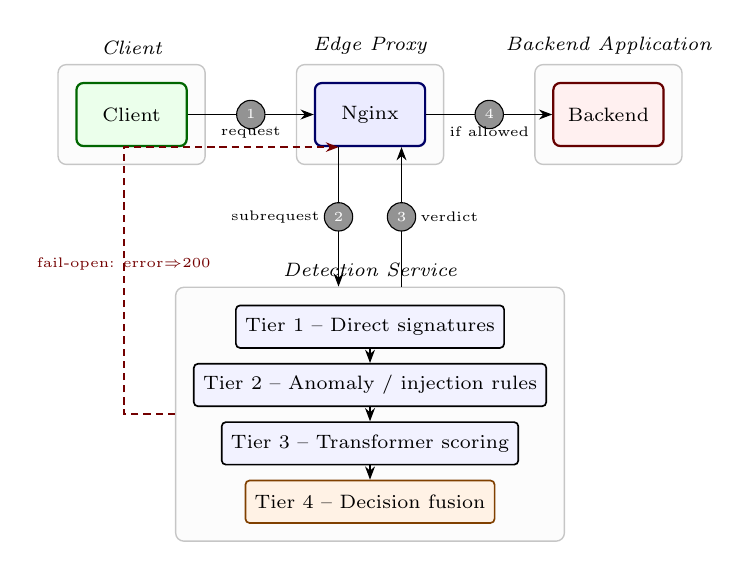
\begin{tikzpicture}[
  node distance=3mm,
  >=Stealth,
  comp/.style={draw,thick,rounded corners=2.5pt,align=center,minimum height=8mm,
              minimum width=14mm,font=\scriptsize,fill=gray!6,
              drop shadow={shadow xshift=0.4pt,shadow yshift=-0.4pt,opacity=0.28}},
  tier/.style={draw,thick,align=center,minimum height=5.4mm,
              minimum width=27mm,font=\scriptsize,fill=blue!5,
              rounded corners=1.5pt,line width=0.6pt},
  tierfusion/.style={tier,fill=orange!10,draw=orange!50!black},
  container/.style={draw,thick,rounded corners=3pt,inner sep=2.2mm,fill=gray!2,
                    draw=gray!45,line width=0.5pt},
  lbl/.style={font=\tiny,align=center},
  badge/.style={draw,circle,fill=gray!85,text=white,font=\tiny,
               inner sep=0pt,minimum size=3.6mm},
  every edge/.style={draw,thick,-{Stealth[length=1.6mm]}}]

  \node[comp,fill=green!8,draw=green!40!black] (client) {Client};
  \node[comp,right=16mm of client,fill=blue!8,draw=blue!40!black] (nginx) {Nginx};
  \node[comp,right=16mm of nginx,fill=red!6,draw=red!40!black] (backend) {Backend};

  \node[tier,below=20mm of nginx,anchor=north] (t1) {Tier 1 -- Direct signatures};
  \node[tier,below=1.8mm of t1] (t2) {Tier 2 -- Anomaly / injection rules};
  \node[tier,below=1.8mm of t2] (t3) {Tier 3 -- Transformer scoring};
  \node[tierfusion,below=1.8mm of t3] (t4) {Tier 4 -- Decision fusion};

  \begin{pgfonlayer}{background}
  \node[container,fit=(t1)(t2)(t3)(t4),
        label={[font=\scriptsize\itshape]above:Detection Service}] (detbox) {};
  \node[container,fit=(nginx),label={[font=\scriptsize\itshape]above:Edge Proxy}] {};
  \node[container,fit=(backend),label={[font=\scriptsize\itshape]above:Backend Application}] {};
  \node[container,fit=(client),label={[font=\scriptsize\itshape]above:Client}] {};
  \end{pgfonlayer}

  \path (client) -- (nginx) coordinate[midway] (m1);
  \path (nginx) -- (backend) coordinate[midway] (m4);

  \draw[->] (client) -- (nginx);
  \node[badge] at (m1) {1};
  \node[lbl,below=1pt of m1] {request};

  \draw[->] (nginx) -- (backend);
  \node[badge] at (m4) {4};
  \node[lbl,below=1pt of m4] {if allowed};

  \draw[->] ([xshift=-4mm]nginx.south) -- ([xshift=-4mm]detbox.north)
        coordinate[pos=0.5] (m2);
  \node[badge] at (m2) {2};
  \node[lbl,left=1.2mm of m2] {subrequest};

  \draw[->] ([xshift=4mm]detbox.north) -- ([xshift=4mm]nginx.south)
        coordinate[pos=0.5] (m3);
  \node[badge] at (m3) {3};
  \node[lbl,right=1.2mm of m3] {verdict};

  \draw[->] (t1) -- (t2);
  \draw[->] (t2) -- (t3);
  \draw[->] (t3) -- (t4);

  \draw[dash pattern=on 2.6pt off 1.8pt,-{Stealth[length=1.6mm]},red!45!black,line width=0.9pt]
    (detbox.west) -- ++(-6.5mm,0) |-
    node[lbl,pos=0.25,above,text=red!45!black,align=center]{fail-open: error$\Rightarrow$200}
    ([xshift=-4mm]nginx.south);
\end{tikzpicture}
\caption{Inline enforcement architecture: the edge proxy issues an internal
sub-request (2) to the detection service container, whose four tiers run in
sequence before a verdict (3) is returned and the request is proxied to the
backend if allowed (4); the backend container only ever sees requests that
passed all four tiers. The dashed path shows the fail-open safeguard: any
unhandled error in the detection path degrades to an allow decision.}
\label{fig:arch}
\end{figure}

\begin{algorithm}[t]
\caption{Decision Fusion (Tier 4)}
\label{alg:fusion}
\begin{algorithmic}[1]
\REQUIRE $(\text{method},\text{uri})$, model score $p$, $\tau_h{=}0.98$, $\tau_\ell{=}0.90$
\STATE $u \gets \text{doubleDecode}(\text{uri})$
\IF{$\text{directSignature}(u)$} \STATE return BLOCK \ENDIF
\STATE $s \gets \text{ruleSignals}(u)$
\IF{$(s.\text{keyword} \wedge s.\text{injection}) \vee s.\text{encoding}$}
   \STATE return BLOCK
\ENDIF
\IF{$p > \tau_h \wedge s.\text{hasSignal}$} \STATE return BLOCK \ENDIF
\IF{$\tau_\ell \le p < \tau_h \wedge (s.\text{keyword} \vee s.\text{charAnom})$}
   \STATE return BLOCK
\ENDIF
\STATE return ALLOW
\end{algorithmic}
\end{algorithm}

Algorithm~\ref{alg:fusion} is equivalent to the closed-form decision rule
\begin{equation}
f(x) =
\begin{cases}
1, & s_{\text{dir}}(u) = 1, \\[2pt]
1, & (s_{\text{kw}} \wedge s_{\text{inj}}) \vee s_{\text{enc}}, \\[2pt]
1, & p(x) > \tau_h \wedge s_{\text{has}}, \\[2pt]
1, & \tau_\ell \le p(x) < \tau_h \wedge (s_{\text{kw}} \vee s_{\text{ca}}), \\[2pt]
0, & \text{otherwise},
\end{cases}
\label{eq:fusion}
\end{equation}
where $u=\text{doubleDecode}(\text{uri})$, $p(x)$ is the model probability
from Eq.~\eqref{eq:softmax}, $s_{\text{dir}},s_{\text{kw}},s_{\text{inj}},s_{\text{enc}},s_{\text{ca}}\in\{0,1\}$
are the Tier~1/2 rule signals (direct signature, keyword, injection
pattern, encoding anomaly, character anomaly), $s_{\text{has}}=s_{\text{kw}}\vee s_{\text{enc}}\vee s_{\text{inj}}\vee s_{\text{ca}}$,
and $f(x)=1$ denotes BLOCK. Discarding the rule-dependent cases
recovers the model-only decision $\hat y(x)$ used for the ``BERT (model
only)'' row of Table~\ref{tab:main}, while discarding the model-dependent
cases recovers the rules-only decision used for that table's ``Rules
only'' row.

\section{Methodology and Setup}

\subsection{Problem Formulation and Preprocessing}
Detection is treated as binary classification over
$x=\texttt{METHOD}\,\Vert\,\texttt{URI}'$, where $\texttt{URI}'$ is the
request path and query string after normalisation. Each request goes
through double URL-decoding to expose anything encoded, contiguous digit
runs get replaced with a single placeholder token so the model does not
latch onto specific identifiers, and the resulting string is tokenised
with the base model's WordPiece vocabulary, capped at $256$ tokens. This
exact preprocessing runs in both the offline evaluation and the deployed
detection service, so the two are guaranteed to see requests the same
way.

Formally, let $\phi(x)\in\mathbb{R}^{256}$ denote the WordPiece token
sequence produced by this preprocessing. The encoder turns $\phi(x)$ into a pooled vector
$h=\mathrm{BERT}(\phi(x))\in\mathbb{R}^{768}$, and a linear head with a
softmax gives the probability that the request is malicious:
\begin{equation}
p(x) \;=\; \frac{\exp(w_1^\top h + b_1)}{\exp(w_0^\top h + b_0) + \exp(w_1^\top h + b_1)},
\label{eq:softmax}
\end{equation}
with $w_0,w_1\in\mathbb{R}^{768}$ and $b_0,b_1\in\mathbb{R}$ the head's
weights and biases for the benign and malicious class. At the default operating point the model-only decision is
$\hat y(x) = \mathbb{1}[p(x)\ge 0.5]$; Section~\ref{sec:threshold}
below instead sweeps this cut-off directly, and Tier~4 (Eq.~\ref{eq:fusion})
combines $p(x)$ with the rule signals rather than thresholding it alone.

\subsection{Model and Training}
Fine-tuning uses \texttt{bert-base-uncased}~\cite{devlin2019bert} with
AdamW, a learning rate of $2{\times}10^{-5}$, batch size $16$, weight
decay $0.01$, a warmup ratio of $0.1$, three epochs, and early stopping
on validation F1. SecureBERT~\cite{aghaei2022securebert,aghaei2025securebert2} and
DistilBERT~\cite{sanh2019distilbert} can be swapped in through the same
training script; comparing encoders is left for future work. We trained on
one NVIDIA Tesla~T4 with PyTorch~2.11 (CUDA~12.8) and Hugging Face
Transformers~4.x, using seed $42$ throughout.

\subsection{Data and Splits}
We train and test on the tabular release of
CSIC~2010~\cite{gimenez2010csic}. The dataset is old, but it is still the
most common public benchmark for HTTP attack detection and the one recent
transformer detectors report on~\cite{wadbert2026,scireports2024novelxsssqli},
which makes comparison possible. SR-BH~2020 and a 2025 ModSecurity audit-log
capture~\cite{modsec30day2025} are used later to check whether the CSIC
results hold on newer traffic. Before splitting, we remove duplicate
requests after normalisation, since CSIC's benign traffic repeats a small
set of templates. This leaves $9{,}492$ unique requests, $68\%$ of them
malicious. These are
split $70/15/15$, stratified by label with a fixed seed of $42$,
giving a $1{,}424$-request held-out test set that never touches training
or model selection.

\subsection{Metrics, Baselines, and Protocol}
We report precision, recall, F1, false-positive rate (FPR) and ROC--AUC.
FPR gets the most attention because, for a WAF, each false positive is a
legitimate user who gets blocked. Writing $\mathrm{TP}$, $\mathrm{FP}$, $\mathrm{TN}$, and
$\mathrm{FN}$ for the counts of true/false positives and negatives on the
held-out test set, the four threshold-dependent metrics are
\begin{equation}
P=\frac{\mathrm{TP}}{\mathrm{TP}+\mathrm{FP}}, \qquad
R=\frac{\mathrm{TP}}{\mathrm{TP}+\mathrm{FN}},
\label{eq:pr}
\end{equation}
\begin{equation}
F_1=\frac{2PR}{P+R}, \qquad
\mathrm{FPR}=\frac{\mathrm{FP}}{\mathrm{FP}+\mathrm{TN}},
\label{eq:f1fpr}
\end{equation}
all evaluated at the decision rule in use (Eq.~\eqref{eq:softmax} at
$\tau=0.5$ for the model alone, or Eq.~\eqref{eq:fusion} for the
hybrid). Unlike $P$, $R$, $F_1$, and FPR, ROC--AUC is not tied to one
operating point: writing $\mathrm{TPR}(\tau)=R$ and $\mathrm{FPR}(\tau)$
for the true- and false-positive rates obtained by thresholding
$p(x)$ at $\tau$, it is the area under the parametric curve traced out
as $\tau$ sweeps from $1$ to $0$,
\begin{equation}
\mathrm{AUC} = \int_0^1 \mathrm{TPR}\bigl(\mathrm{FPR}^{-1}(t)\bigr)\,dt,
\label{eq:auc}
\end{equation}
which is what makes it a threshold-independent summary of ranking
quality, in contrast to the other four metrics reported at a single
$\tau$. For baselines, the evaluation
uses the deterministic rule engine on its own (Tiers~1--2) and TF--IDF
character-$n$-gram features feeding a linear SVM and a random forest.
Four protocols structure the results:
\emph{within-dataset} detection on the CSIC~2010 splits, an
\emph{ablation} comparing rules-only, model-only, and the full hybrid on
the same test set, a \emph{threshold-sensitivity} sweep over the model's
decision threshold, and an \emph{adversarial} evaluation that mutates
blocked payloads using six semantics-preserving transformations.

\section{Results}
Every number below comes from the held-out CSIC~2010 test split
($n=1{,}424$).

\subsection{Detection and Ablation}
Table~\ref{tab:main} gives the detection results. BERT (F1~$0.949$,
FPR~$0.064$, AUC~$0.974$) is slightly behind the TF--IDF SVM (F1~$0.965$,
FPR~$0.057$), ahead of the random forest, and far ahead of the rule engine,
which catches $43.5\%$ of attacks at $20.9\%$ FPR. The hybrid blocks when
either the rules or the model fire, so it also takes on the rules' false
positives: F1 falls to $0.849$ and FPR rises to $0.229$. Compared with the
model alone, the hybrid loses about $16.5$ points of true-negative rate and
$11.2$ points of recall on CSIC~2010. Section~\ref{sec:crossdataset} shows
that this changes on other traffic.

\begin{table}[t]
\centering
\caption{Detection and Ablation on CSIC 2010 (Test)}
\label{tab:main}
\begin{tabular}{@{}lccccc@{}}
\toprule
Method & P & R & F1 & FPR & AUC \\
\midrule
Rules only            & 0.816 & 0.435 & 0.567 & 0.209 & --- \\
TF--IDF + SVM         & 0.973 & 0.957 & 0.965 & 0.057 & 0.992 \\
TF--IDF + RF          & 0.929 & 0.924 & 0.927 & 0.150 & 0.958 \\
BERT (model only)     & 0.969 & 0.930 & 0.949 & 0.064 & 0.974 \\
Hybrid (proposed)         & 0.884 & 0.817 & 0.849 & 0.229 & 0.974 \\
\bottomrule
\end{tabular}
\end{table}

\subsection{Per-Attack-Class Recall}
Let $\mathcal{X}_a=\{x : y(x)=1,\ \mathrm{type}(x)=a\}$ be the malicious
test requests belonging to attack category $a\in\{\text{sqli},
\text{encoding},\text{other}\}$. Per-class recall is Eq.~\eqref{eq:pr}'s
$R$ restricted to that subset,
\begin{equation}
R_a = \frac{1}{|\mathcal{X}_a|}\sum_{x\in\mathcal{X}_a} \mathbb{1}[f(x)=1],
\label{eq:perclass}
\end{equation}
so that $R=\sum_a |\mathcal{X}_a| R_a / \sum_a |\mathcal{X}_a|$ recovers
the overall recall in Table~\ref{tab:main} as the size-weighted average
of the per-class values. The hybrid detects every SQL-injection and encoding attack in the test set
($1.00$ recall for each), while the mixed ``other'' group reaches $0.764$;
the model alone shows the same order. SQLi and encoded payloads contain
clear keywords and structure, whereas the ``other'' group lacks a common
pattern, so both detectors find it hardest.

\subsection{Threshold, Latency, and Adversarial Robustness}
\label{sec:threshold}
Raising the model's decision threshold from $0.50$ to $0.98$ lowers recall
from $0.930$ to $0.880$ and cuts FPR from $0.064$ to $0.026$.
Single-request GPU inference costs a median
of $12.7$~ms ($p99{=}18.2$~ms), and throughput follows directly from
the mean per-request latency $\bar\ell$ (in milliseconds) for a single
inference process,
\begin{equation}
\mathrm{RPS} = \frac{1000}{\bar\ell},
\label{eq:rps}
\end{equation}
giving the $82$ requests per second per process reported in
Table~\ref{tab:latency}, fast enough to sit inline. For the adversarial
test, let $B\subset\mathcal{X}_{\text{mal}}$ be the malicious requests
initially blocked by a given configuration and $m:\text{URI}\to\text{URI}$
one of the six semantics-preserving mutations; its evasion rate against
that configuration's decision function $g$ (either $f$ from
Eq.~\eqref{eq:fusion} or $\hat y$) is
\begin{equation}
E_m = \frac{1}{|B|}\sum_{x\in B} \mathbb{1}[g(m(x))=0],
\label{eq:evasion}
\end{equation}
i.e.\ the fraction of originally-blocked payloads that flip to
ALLOW after mutation, averaged over the six $m$ to give the
overall figures in Table~\ref{tab:latency}. Four of the six mutations ($E_m=0$) never changed
a verdict for either configuration. The other two, an inline SQL comment
and a junk query parameter, each evaded the model alone on $0.36\%$ of
blocked payloads ($0.12\%$ overall); none of the six evaded the hybrid
(Table~\ref{tab:latency}). This is far lower than the bypass rates
WAF-A-MoLE~\cite{demetrio2020wafamole} and AdvSQLi~\cite{advsqli2024}
report against ML-based WAFs, but a $0.12\%$ difference cannot justify the
hybrid's much higher FPR; the cross-dataset results below are more
informative.

\begin{table}[t]
\centering
\caption{Inline Latency (Tesla T4) and Adversarial Evasion (6 Mutation Families)}
\label{tab:latency}
\begin{tabular}{@{}lcccc@{}}
\toprule
Config & p50 (ms) & p99 (ms) & RPS & Evasion \\
\midrule
BERT (model only) & 12.7 & 18.2 & 81.7 & 0.0012 \\
Hybrid & --- & --- & --- & 0.00 \\
\bottomrule
\end{tabular}
\end{table}

\subsection{Cross-Dataset Generalisation}
\label{sec:crossdataset}
All results so far use CSIC~2010 for both training and testing. We next
applied the CSIC-trained model, without retraining, to
SR-BH~2020~\cite{srbh2020} (Table~\ref{tab:crossdataset}). These numbers come from an earlier
fine-tuning run, so the reference row differs slightly from
Table~\ref{tab:main}; the qualitative pattern does not depend on the run. On SR-BH the model alone labels almost every request as malicious
(FPR~$1.00$), so F1 falls to $0.601$ although recall is perfect. The hybrid,
on the same requests, reaches FPR~$0.001$ and F1~$0.971$. Seen in isolation,
this supports the rule layer, since the false positives it adds on
CSIC~2010 are repaid once the traffic changes. A similar collapse has been reported for network
intrusion detectors moved between
networks~\cite{cantone2024crossdataset,venkatesan2026crossdataset}.
Section~\ref{sec:thirdcorpus}, however, shows that the rule layer does not
help on a second corpus.

\begin{table}[t]
\centering
\caption{Zero-Shot Cross-Dataset Transfer: CSIC-Trained Detector on SR-BH~2020}
\label{tab:crossdataset}
\begin{tabular}{@{}lccccc@{}}
\toprule
Configuration & P & R & F1 & FPR & AUC \\
\midrule
CSIC $\to$ CSIC (reference) & 0.979 & 0.953 & 0.966 & 0.044 & 0.986 \\
CSIC $\to$ SR-BH (model only) & 0.429 & 1.000 & 0.601 & 1.000 & 0.859 \\
CSIC $\to$ SR-BH (hybrid) & 0.999 & 0.944 & 0.971 & 0.001 & 0.859 \\
\bottomrule
\end{tabular}
\end{table}

\subsection{A Second Corpus Where the Rule Layer Hurts Instead}
\label{sec:thirdcorpus}
The second test corpus holds thirty days of 2025 production requests blocked
by a deployed ModSecurity instance~\cite{modsec30day2025}. It contains
attacks only, so we report recall alone (Table~\ref{tab:thirdcorpus}).
Here the pattern is reversed. The model alone keeps a recall of $0.999$,
while the hybrid drops to $0.151$ and misses about five of every six
attacks the model catches. We attribute this to the high-confidence branch
of Eq.~\eqref{eq:fusion} ($p(x){>}\tau_h \wedge s_{\text{has}}$), which
blocks only when a rule signal accompanies the model score. The keyword and
signature lists behind $s_{\text{has}}$ were written for CSIC-era payloads;
on the 2025 requests the model is confident but the rule signal is often
absent, so the branch does not fire. On SR-BH the rules add coverage; here they hold back correct model
decisions because the rule condition no longer matches. Taken together,
Tables~\ref{tab:crossdataset} and~\ref{tab:thirdcorpus} show that the effect
of the rule layer on generalisation depends on the corpus, so an operator
should check it on their own traffic before relying on it.

\begin{table}[t]
\centering
\caption{Zero-Shot Recall on a Second Corpus: Real 2025 Production Traffic (Attack-Only)}
\label{tab:thirdcorpus}
\begin{tabular}{@{}lc@{}}
\toprule
Configuration & Recall \\
\midrule
CSIC $\to$ ModSecurity-2025 (model only) & 0.999 \\
CSIC $\to$ ModSecurity-2025 (hybrid) & 0.151 \\
\bottomrule
\end{tabular}
\end{table}

\section{Discussion}
\label{sec:discussion}
Table~\ref{tab:compare} shows that none of the compared works combines
inline latency, false-positive cost, evasion, and cross-dataset testing.
A TF--IDF SVM still edges the transformer on in-corpus F1 and FPR, so the
transformer's case rests on robustness and deployability.

The results do not favour one design throughout. The model alone resists
four of six mutation families fully and is evaded $0.12\%$ of the time,
against $0\%$ for the hybrid, so robustness explains little of the
hybrid's extra false positives. On SR-BH~2020 the rule layer turns a model
with FPR~$1.00$ into a hybrid with F1~$0.971$; on the 2025 corpus it reduces
a recall of $0.999$ to $0.151$, because its high-confidence branch needs a
rule signal that the newer payloads rarely trigger. Which effect appears
depends on the corpus, and nothing we measured predicts it in advance.
For deployment, the SR-BH result alone is not a reason to trust the rule
layer in general; operators should test on their own traffic or update the
rule signals whenever the model is retrained. Rule brittleness, the reason
for using a learned detector in the first place (rules alone give $20.9\%$
FPR), shows up on both sides: as extra false positives on CSIC~2010 and
SR-BH, and as missed coverage on the 2025 corpus. Our F1 of $0.949$ is below
the $>$99\% reported in~\cite{wadbert2026,scireports2024novelxsssqli}. We
believe part of this gap comes from deduplication, because without it
near-identical CSIC requests can fall on both sides of the split.

This study has several limitations. Transfer was tested only from CSIC to
the other corpora, not in reverse. The main results come from one
fine-tuning run, and a second run with the same seed gave F1 $0.966$
instead of $0.949$. The 2025 corpus has no benign traffic, so only recall
can be computed, and six mutation families do not cover every evasion
technique. The detector reads the request line and body but not responses,
so it says nothing about data exfiltration. Fail-open favours availability
over security, so its activation rate should be monitored. Latency was
measured on a GPU only; CPU and DistilBERT setups have not been benchmarked.

\section{Conclusion}
We placed a fine-tuned transformer in the request path of a WAF using
Nginx sub-request authorization and measured its cost and accuracy. On
CSIC~2010 the model reaches F1~$0.949$ at $6.4\%$ FPR with a median
inference time of $12.7$~ms. Adding the rule layer lowers F1 to $0.849$ and
raises FPR to $22.9\%$ on the same data, and its small gain in mutation
resistance does not offset that. On unseen traffic the rule layer helped on
SR-BH~2020 and hurt on 2025 production traffic
(Sections~\ref{sec:crossdataset} and~\ref{sec:thirdcorpus}), so operators
should test it on their own traffic. Future work covers transfer in the
reverse direction, updating the rule signals for the 2025 corpus, and a
calibrated fusion rule.

\footnotesize
\bibliographystyle{IEEEtran}
\bibliography{references}

\end{document}
